%!TEX root=../main.tex
\section{System Architecture}
\label{sec:architecture}
\begin{figure}
    \centering
    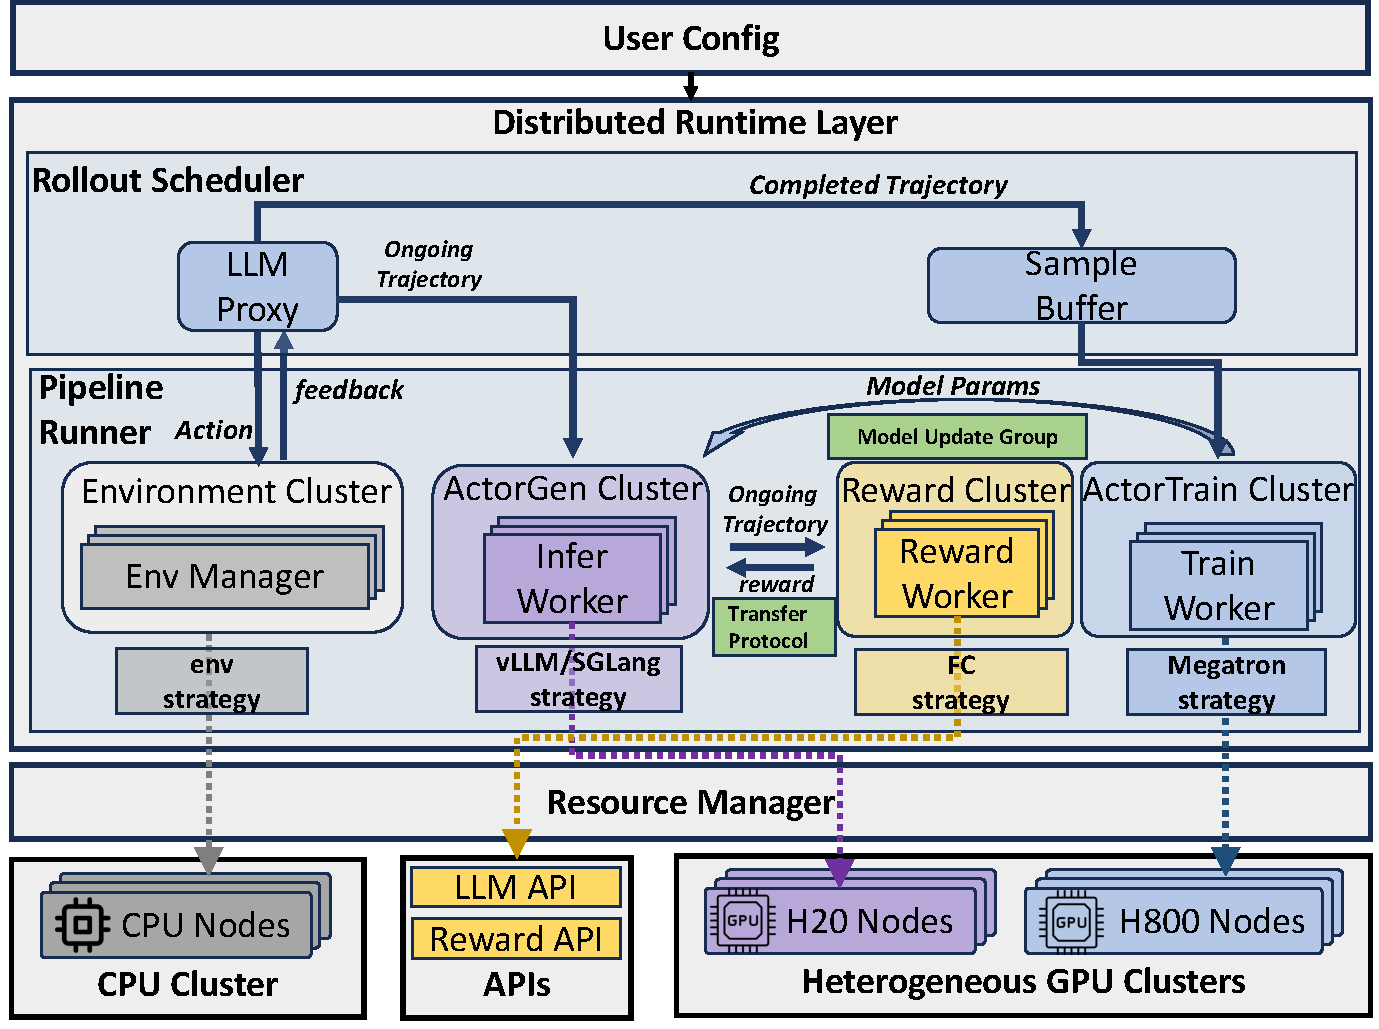
\includegraphics[width=0.9\linewidth]{figs/overview/sys_arch_osdi_updated.pdf}
    \caption{System Architecture of \SystemName{}}
    \label{fig:sys_arch}
\end{figure}


We implemented \SystemName{} in approximately 60k lines of Python code. 
\autoref{fig:sys_arch} shows the architecture of \SystemName{} consisting of the distributed runtime layer and the resource manager.
\SystemName{} parses user configurations and constructs the training pipeline atop the distributed runtime. The runtime includes a rollout scheduler that manages the rollout execution workflow and the \texttt{Cluster} runtime that performs distributed computation and communication. The resource manager allocates heterogeneous resources from a shared  pool to the workers.

\noindent\textbf{Rollout Scheduler.} It controls the rollout stage via managing the lifecycle of each trajectory. The \texttt{LLMProxy} interacts with multiple environment managers and routes ongoing trajectories to appropriate inference workers. Completed trajectories are added to \texttt{SampleBuffer} for subsequent model training. 


\noindent\textbf{Pipeline Runner.} The pipeline runner consists of multiple \texttt{Cluster}s that assume different roles in agentic RL training (e.g., reward, environment). Each \texttt{Cluster} orchestrates a collection of workers to perform a specific type of distributed computation (e.g., training, generation, environment interaction) using a chosen strategy (e.g., vLLM~\cite{vllm}, Megatron~\cite{shoeybi2019megatron}, Function Compute~\cite{alibaba_function_compute}). 
% \texttt{Cluster}s exchange trajectories via a transfer protocol, with trajectories represented as \texttt{ObjRef} objects provided by Ray~\cite{ray}, enabling deferred object materialization and hiding data transmission overhead.
\texttt{Cluster}s exchange trajectories via Ray's \texttt{ObjRef}s~\cite{ray}, which enables deferred materialization and hides data transmission overhead by passing object references instead of data copies.
For model weight synchronization, each \texttt{Cluster} exposes a \texttt{model\_update\_group} interface that leverages high‑throughput transfer engines such as NCCL~\cite{nccl} and Mooncake~\cite{qin2024mooncake}, utilizing NVLink, InfiniBand, and Ethernet to efficiently synchronize weights.

\noindent\textbf{Resource Manager.} The resource manager uses a persistent metadata store to maintain a real-time view of critical state, including the distributed runtime state, cluster resource availability, and service API availability. When it receives a worker deployment request, it first consults the metadata store to validate the request, then binds the requested resources or external services to the workers.

